\section{Глава 1}

\subsection{Теоретические основы}

В данной работе нам понадобится ряд формальных определений и терминов, которые мы будем использовать в дальнейшем. 

\subsubsection{Понятие подпрограммы}

Первым делом, условимся использовать термины \term{подпрограмма}, \term{функция}, \term{метод}, \term{процедура} взаимозаменяемо, в смысле, интуитивно соответствующему англ. \eng{callable}. Более формально:

\begin{definition}
    \term{Подпрограммой} (функцией, методом, процедурой) будем называть выделенную последовательность инструкций, в которую может быть передано управление, и которая по завершению возвращает его в место вызова \cite{Wheeler52}.
\end{definition}

Отметим, что также в это определение укладываются все объекты, на которых можно произвести непосредственный вызов, если таковые поддерживаются языком -- например, объекты, с переопределенным методом \code{invoke} в \lang{Kotlin}, \code{apply} в \lang{Scala}, \code{\_\_call\_\_} в \lang{Python} и т.д.





\subsubsection{Понятие эффекта и системы эффектов}

Центральным определением в данной работе, является, разумеется, \term{эффект}. Однако несмотря на то, что это определение, судя по всему, было введено еще на заре развития программирования (так, ранние работы по аксиоматизации программирования уже ссылаются на этот термин без отдельного его введения \cite{Hoare69, Schwartz67}), общепринятой формулировки за все это время не появилось. 

В классических источниках, под эффектом чаще всего понимают <<некоторое видимое изменение в окружении>> \cite{Luc88}, или даже еще более конкретно <<изменение в памяти программы>> \cite{Vak09}. Некоторые исследователи и вовсе ограничивают это определение до <<чтения или записи в изменяемое состояние программы>> \cite{Green99}. Это можно резюмировать следующим образом:

\begin{definition}
\label{def-effect-1}
    \term{Эффектом} называется некоторое изменение, производимое подпрограммой в состоянии вычислителя (кроме возвращения подпрограммой значения).
\end{definition}

Другие же авторы употребляют более широкую трактовку <<эффекта>> \cite{Nielson99}: 

\begin{definition}
\label{def-effect-2}
    \term{Эффектом} является описание действий, происходящих в ходе выполнения подпрограммы.
\end{definition}

Разумеется, формулировка \ref{def-effect-2} является слишком широкой -- вплоть до того, что под нее подходит непосредственно исходный код тела функции. С другой же стороны, формулировка \ref{def-effect-1} является нежелательно узкой в контексте данной работы. Поясним это на примере. 

Рассмотрим следующую функцию, которая является тривиальной оберткой над проверкой переменной на принадлежность строковому типу:

\begin{minted}{kotlin}
fun isString(x: Any?): Boolean {
    return (x is String)
}
\end{minted}

И рассмотрим следующий участок кода:

\begin{minted}{kotlin}
if (isString(t)) {
    ...
}
\end{minted}

Мы хотели бы сказать, что в истинной ветке условного оператора мы наблюдаем тот эффект, что <<\code{isString} вернула значение \code{true}>>. Однако это действие не подходит под определение эффекта \ref{def-effect-1}. Мы могли бы отказаться от специального случая для возвращаемых значений в этой формулировке, но в дальнейшем мы встретим некоторые утверждения, которые мы тоже хотели бы называть эффектами, но которые не описывают вообще никакого изменения в состоянии вычислителя.

Поэтому нам понадобится определение, чуть более слабое, чем определение \ref{def-effect-1}, но при этом не являющееся чересчур расплывчатым, как \ref{def-effect-2}. Мы сформулируем его следующим образом:

\begin{definition}
    \label{def-effect}
    \term{Эффект} -- это некоторая информация об окружении, получаемая при выполнении подпрограммы.
\end{definition}

Т.к. это определение рассматривает только окружение, то сразу отпадают все слишком широкие его интерпретации. В частности, все, что подпрограмма делает со своими локальными переменными, не подходит под это определение -- что очень удобно, т.к. изменения в локальных переменных нас никоим образом не интересуют.

С другой стороны, это определение включает в себя определение \ref{def-effect-1}, т.к. <<изменение в состоянии>>, несомненно, является <<информацией об окружении>>.

Наконец, как мы увидим чуть позже, под это определение подходят и довольно нестандартные действия, которые нам будет удобно считать эффектами во имя общности подхода.


\bigskip

Естественным продолжением определения эффекта является определение \term{системы эффектов}. Само по себе название уже достаточно интуитивно, особенно если провести параллель <<эффект также относится к системе эффектов, как тип относится к системе типов>>. Тем не менее, мы дадим здесь формальное определение, т.к. это понятие также является центральным в данной работе и будет многократно использоваться в дальнейшем:

\begin{definition}
    \term{Система эффектов} -- это множество правил, по которым подпрограммам и их конкретным вызовам приписываются эффекты, и по которым осуществляется взаимодействие эффектов.
\end{definition}




\subsubsection{Анализ потока данных}

Кроме того, нам в дальнейшем нам понадобятся основные концепции data-flow анализа.

Начнем с понятия графа потока управления (англ. \eng{control-flow graph, CFG}) Каждая инструкция в нем представлена одной вершиной, и если между вершинами $u$ и $v$ есть ребро, то это означает что после инструкции $u$ управление может быть передано 
в инструкцию $v$. 

Рассмотрим простой пример кода:

\begin{minted}{kotlin}
    if (x == 0) {
        println("True branch")
    } else {
        println("False branch")
    }
    println("If-end")    
\end{minted}

Ему соответствует граф потока управления, как на рисунке \ref{control-flow-example}

\begin{figure}
    \centering
    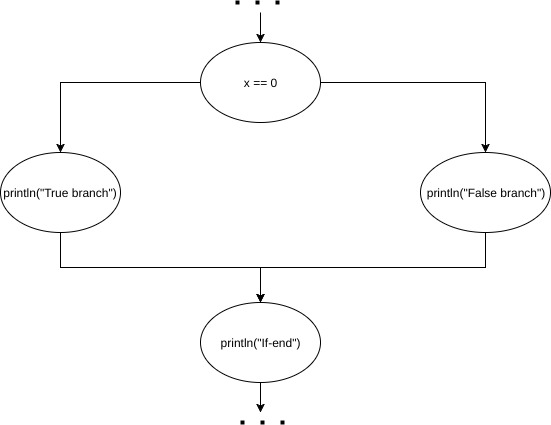
\includegraphics[scale=0.5]{img/control-flow-example}
    \caption{Пример графа потока управления}
    \label{control-flow-example}
\end{figure}


Так, после инструкции, вычисляющей условие в \code{if}, поток управления раздвоился, отражая тот факт, что мы не можем знать при статическом анализе (без дополнительных предположений), какая из веток выполнится. После ветки вновь сливаются в один поток, как и следовало ожидать.

Разумеется, граф потока управления не обязан быть ацикличным -- конструкции \code{for}, \code{while}, \code{goto} (безусловных переход) могут вносить в него обратные ребра.

Важно заметить, что любому возможному пути исполнения в программе обязательно соответствует некоторый путь в CFG, но обратное не верно. Например, путь может проходить через истинную ветку выражения \linebreak \code{if (x == 0) } и через истинную ветку выражения \code{if (x != 0)}, хотя между первым и вторым оператором могло и не быть никаких изменений переменной \code{x}, и иногда это даже можно доказать статически.
Тем не менее, это не нарушает консервативности анализа, поскольку при анализе будет обязательно рассмотрен любой реально возможный путь исполнения. 

Конструкция графов потока управления сама по себе позволяет обнаружить совсем простые ошибки, вроде недостижимого кода из-за неправильного использования безусловных переходов. Однако она становится особо мощной и полезной, если использовать ее вместе с концепцией анализа потока данных.

\begin{definition}
	Анализ потока данных (англ. \eng{data-flow analysis})  -- это метод статического анализа, который основывается на извлечении информации из характеристик и свойств потока данных вдоль различных путей исполнения в программе.
\end{definition}

Основная идея основывается на наблюдении, что в любой момент времени при выполнении программы существует некоторое глобальное состояние, которое состоит из множества всех переменных, их значений, а также другой информации, зависящей от конкретного типа анализа (например, счетчик количества вызовов для функций, статус инициализации переменной, и т.д.). Тогда для каждой точки программы можно ввести понятие \term{значения потока данных} (от англ. \eng{data-flow value}), которое является абстракцией всех возможных глобальных состояний, которые можно наблюдать в данной точке. Для краткости, в дальнейшем мы будем писать DFV вместо <<значение потока данных>>.

В силу того, что потенциально количество возможных путей исполнения в программе может быть бесконечно \cite{dragon-book}, на практике делается два упрощения: во-первых, конкретное DFV не хранит историю, как управление могло придти к этой точке программы, а во-вторых, в зависимости от конкретного анализа, откидывается некоторая излишняя информация. Так, например, при анализе инициализации переменных, нам не важно, какие значения может иметь переменная, и на каких путях исполнения они могли быть получены. Достаточно знать, правда ли, что на любом пути исполнения, достигающем данную точку, данная переменная была инициализирована, или нет. Таким образом, для каждой переменной достаточно просто хранить бинарный флаг, что значительно упрощает реализацию на практике.

Далее, каждой инструкции $s$ соответствует \term{входное состояние} -- глобальное состояние непосредственно перед выполнением инструкции, которое мы будем обозначать $in[s]$, и \term{выходное состояние} -- соответственно, глобальное состояние непосредственно после выполнения инструкции (его мы будем обозначать $out[s]$). Обратим внимание, что выходное состояние для одной инструкции является входным для следующей, с котором она соединена ребром в CFG. Каждому входному (выходному) состояние соответствует некоторое DFV, и в силу предыдущего факта, это отображение является сюръекцией, но не биекцией.

Кроме того, каждая инструкция задает некоторое преобразование, называемое \term{функцией перехода} (англ. \eng{transfer function}), которое по входному состоянию выдает выходное. Конкретный вид преобразования определяется анализом и самой инструкций. 

Таким образом, мы получаем набор уравнений на переменные $in[x]$, $out[x]$ для всех $x \in I$, где $I$ -- множество инструкций в программе. Хотелось бы получить некоторое решение этих уравнений, т.е. множество значений для входных-выходных состояний, удовлетворяющее этим уравнениям. Мы не будем вдаваться в подробности того, как это делается, т.к. это иррелевантно к данной работе, подробней про методы решения систем уравнений на поток данных можно прочитать в канонических источниках: \cite{dragon-book, muchnick}. В дальнейшем нам будет достаточно концепции графа потока управления, входных-выходных состояний и функций перехода.



\newpage

\subsection{Предметная область}

Для того, чтобы получить конкретную почву для дальнейших рассуждений и ограничить область рассматриваемых проблем, мы здесь приведем несколько имеющихся на данный момент проблем со статическим анализом в языке \lang{Kotlin}. 



\subsubsection{Механизм умных приведений типов}

Важным механизмом, понимание которого необходимо для дальнейшего разговоре о \lang{Kotlin}, является механизм \term{умных приведений типов} (англ. \eng{smartcasts}). 

Очень часто, перед явным приведением типа в коде выполняется проверка на подтип (для того, чтобы такое приведение было безопасным). В \lang{Java} это выглядит примерно следующим образом:

\begin{minted}{java}
    if (x instanceof string) {
        string s = (string) x;
        ... usage of s ...
    }
\end{minted}

Суть механизма умных приведений типов заключается в том, чтобы облегчить программисту жизнь и выполнить приведение к более частному типу автоматически там, где это безопасно. 

Вот эквивалентный участок кода на \lang{Kotlin}: 

\begin{minted}{kotlin}
    if (x is String) {
        val len = x.length
    }
\end{minted}

Во второй строке произошло автоматические приведение типа, благодаря чему стал возможным доступ к полю \code{String.length}.

Особенно удобно это вместе с \code{when}-конструкцией, которая является более мощным аналогом \code{switch-case} из \code{Java}, в частности, позволяя использовать в \code{Kotlin} синтаксис, напоминающий сравнение с образцом (англ. \code{pattern matching}).

\begin{minted}{kotlin}
    when (x) {
        is String -> x.length   // x casted to String
        is List<Int> -> x.size  // x casted to List
        is Double -> x * 2.0    // x casted to Double
        
    }
\end{minted}




\subsubsection{Проблемы механизма умных приведений типов}

Основная проблема заключается в том, что анализ возможности приведения типа выполняется без учета межпроцедурных взаимодействий. Так, давайте вспомним уже знакомую нам функцию проверки на строковый тип:

\begin{minted}{kotlin}
    fun isString(x: Any?): Boolean {
        return x is String
    }
\end{minted}

Теперь если использовать эту функцию в качестве условия условного оператора, то умное приведение типа выполнено не будет:

\begin{minted}{kotlin}
    if (isString(x)) {
        val s = x as String    // explicit cast needed
    }
\end{minted}

Особенно актуальна эта проблема для работы с коллекциями с использованием stream-like API, предоставляемом в \lang{Kotlin}. Так, существует метод \code{filter}, который оставляет в коллекции только те элементы, на которых переданный предикат вернул \code{true}. Этот метод довольно часто используется для того, чтобы оставить в коллекции только объекты определенного типа: \code{list.filter(x -> x is String)} оставит в коллекции \code{list} только строки.

Разумеется, в обоих описанных случаях компилятор не может просто так выполнить умное приведение типа -- для этого ему нужно знать некоторый <<контракт>> вызываемой функции. 

Для \code{isString} нужно знать, что <<\code{isString(x)} возвращает \code{true} тогда и только тогда, когда \code{x} -- \code{String}>>. 

Для \code{filter} нужно знать, что он оставляет в коллекции только те объекты, на которых переданный предикат вернул \code{true}.


\bigskip

Другим распространенным случаем, когда умное приведение типов можно было бы сделать, но оно не делается, являются функции, которые могут завершиться с исключением. 

Рассмотрим следующий пример:

\begin{minted}{kotlin}
    assert(x is String)
    val s = x as String    // explicit cast needed
\end{minted}

Если мы будем считать, что \code{assert} бросает исключение всегда, когда его условие -- \code{false} (на практике это зависит от ключей окружения, но мы опустим эти детали реализации), тогда во второй строке автоматическое приведение типа может быть безопасно выполнено. Тем не менее, на данный момент компилятор \lang{Kotlin} этого не делает, ровно по тем же причинам, что и в примерах выше -- он не выполняет межпроцедурного анализа, и потому ему не известен контракт <<assert>>. 




\subsubsection{Анализ инициализации переменных}

\lang{Kotlin} поддерживает отложенную инициализацию локальных переменных и будет отслеживать и предупреждать об использовании неинициализированных переменных:

\begin{minted}{kotlin}
    val x: Int
    // println(x)
    x = 5
    println(x)
\end{minted}

Если раскомментировать строку 2, то компилятор вполне законно выдаст ошибку об использовании неинициализированной переменной. 

Теперь рассмотрим функцию \code{run}, которая просто вызывает переданную ей лямбду: 
\begin{minted}{kotlin}
    fun run(block: () -> Unit): Unit {
        block()
    }
\end{minted}

Если теперь выполнить отложенную инициализацию переменной внутри лямбды, переданной внутрь \code{run}, то компилятор уже не сможет доказать, что переменная была корректно проинициализированна:

\begin{minted}{kotlin}
    val x: Int
    run ({ () -> x = 5 })
    println(x)
\end{minted}

Компилятор отвергает подобный код, ошибочно сообщая об использовании неинициализированной переменной в строке 3. Причина этого примерно такая же, как и во всех предыдущих примерах: компилятор не знает контракта функции \code{run}, и потому не знает, что лямбда \code{\{ () -> x = 5 \}} будет гарантированно вызвана.

Этот пример умышленно утрирован для простоты объяснения. На самом деле, это вполне актуальная и серьезная проблема, т.к. \code{Kotlin} придерживается философии введения как можно меньшего количества ключевых слов. Это возможно из-за существования лямбд и функций высшего порядка, а также из-за синтаксического сахара, позволяющего передавать лямбду в виде блока, если она передается последней в списке параметров. Именно так реализован аналог ключевого слова \code{synchronized} из \lang{Java}: в \lang{Kotlin} это обычная функция, определенная примерно следующим образом (детали взятия и освобождения блокировки опущены для ясности).

\begin{minted}{kotlin}
    fun synchronized(block: () -> Unit): Unit {
        ... take lock ...
        block()
        ... release lock ...
    }
\end{minted}

В пользовательском коде использование этой функции с учетом описанного выше синтаксического сахара выглядит следующим образом:

\begin{minted}{kotlin}
    val x: Int
    synchornized {
        x = 5
    }
    println(x)
\end{minted}

Точно также, как в примере с \code{run}, компилятор заявляет о том, что в строке 5 переменная \code{x} не инициализирована. Это уже более серьезная проблема, т.к. здесь нельзя обойтись парой избыточных символов, как это было в примере с умными приведениями типа. 

Такой случай использования является вполне жизненным и распространенным, и в будущем будет появляться лишь больше функций, похожих на \code{run} и \code{synchronized} (так, на момент написания этой работы уже добавлена экспериментальная поддержка корутин, которые используют точно такую же парадигму).

Для того, чтобы решить это проблему, необходимо некоторым образом донести до компилятора контракт всех таких функций: что они вызывают переданную им лямбду некоторое статически детерминированное число раз. 



\subsubsection{Анализ}

Подведем краткий итог проблем, которые мы пронаблюдали в предметной области:

\begin{itemize}
    \item Корнем всех перечисленных выше проблем являются неучтенные межпроцедурные взаимодействия
    
    \item Для того, чтобы корректно дополнить анализ, необходимо извлечь некоторые факты и утверждения о том, как именно работают функции (связь входного и выходного значения, как в \code{isString}, или же информация о поведении функции по отношению к переданным аргументам, как в \code{run})
    
    \item Следует ожидать, что контракты могут становиться весьма нетривиальными, равно как и то, что достаточно простые контракты может оказаться непросто выводить в автоматическом режиме (например, функция может действительно вызывать лямбду ровно один раз, но при этом делать еще множество других нетривиальных вещей, тем самым затрудняя анализ).
\end{itemize}

Таким образом, мы интересуемся некоторыми системами, облегчающими межпроцедурный анализ за счет использования знания о том, как функция взаимодействует с окружением. Кроме того, хотелось бы, чтобы такие системы позволяли пользователю прописать вручную контракты в местах, где автоматический вывод не справляется.

Если внимательно посмотреть на эту формулировку, то можно заметить, что это практически определение систем эффектов. Тем не менее, в следующем разделе мы рассмотрим еще некоторых систем, которые решают практически ту же проблему, и проведем их сравнительный анализ.

